
The results obtained on the test images are summarized in Table~\ref{Results:tab:images}, while some qualitative results are shown in Figure~\ref{Results:fig:images}.

\begin{table}[H]
\centering
\begin{tabular}{c|c|c|c|c}
\toprule
\textbf{Images} & \textbf{mIoU} & \textbf{Accuracy} & \textbf{Predicted sum} & \textbf{Sum error} \\[4pt]
\midrule
image a     & $0.915$     & $92.86\,\%$     & $8.87$     & $-0.10$ \\[8pt]
image b     & $0.966$     & $100.0\,\%$     & $4.92$     & $ 0.00$ \\[8pt]
image c     & $0.838$     & $100.0\,\%$     & $4.72$     & $+0.20$ \\[8pt]
image d     & $0.836$     & $81.25\,\%$     & $9.28$     & $-0.79$ \\
\bottomrule
\end{tabular}
\caption{Performance metrics for test images.}
\label{Results:tab:images}
\end{table}

In these images the algorithm is able to correctly recognize almost every coin, with an average accuracy of $93.53\,\%$.
The light conditions have a strong impact on the performance of the algorithm, as shown by the results on Figure~\ref{Results:fig:image0}~\ref{Results:fig:image3}, where the $10$ cent coin is not detected due to the strong reflections on its surface.
The only false positive is instead present in Figure~\ref{Results:fig:image2}, where a lira is confused with a $20$ cent coin.

Summing up the predicted values, the total estimated amount is $27.79$ euros, with an error of $-0.69$ euros which corresponds to a relative error of $-2.43\,\%$ from the ground truth value of $28.48$ euros.

\begin{figure}[H]
    \centering
    \subfloat[\label{Results:fig:image0}]{
        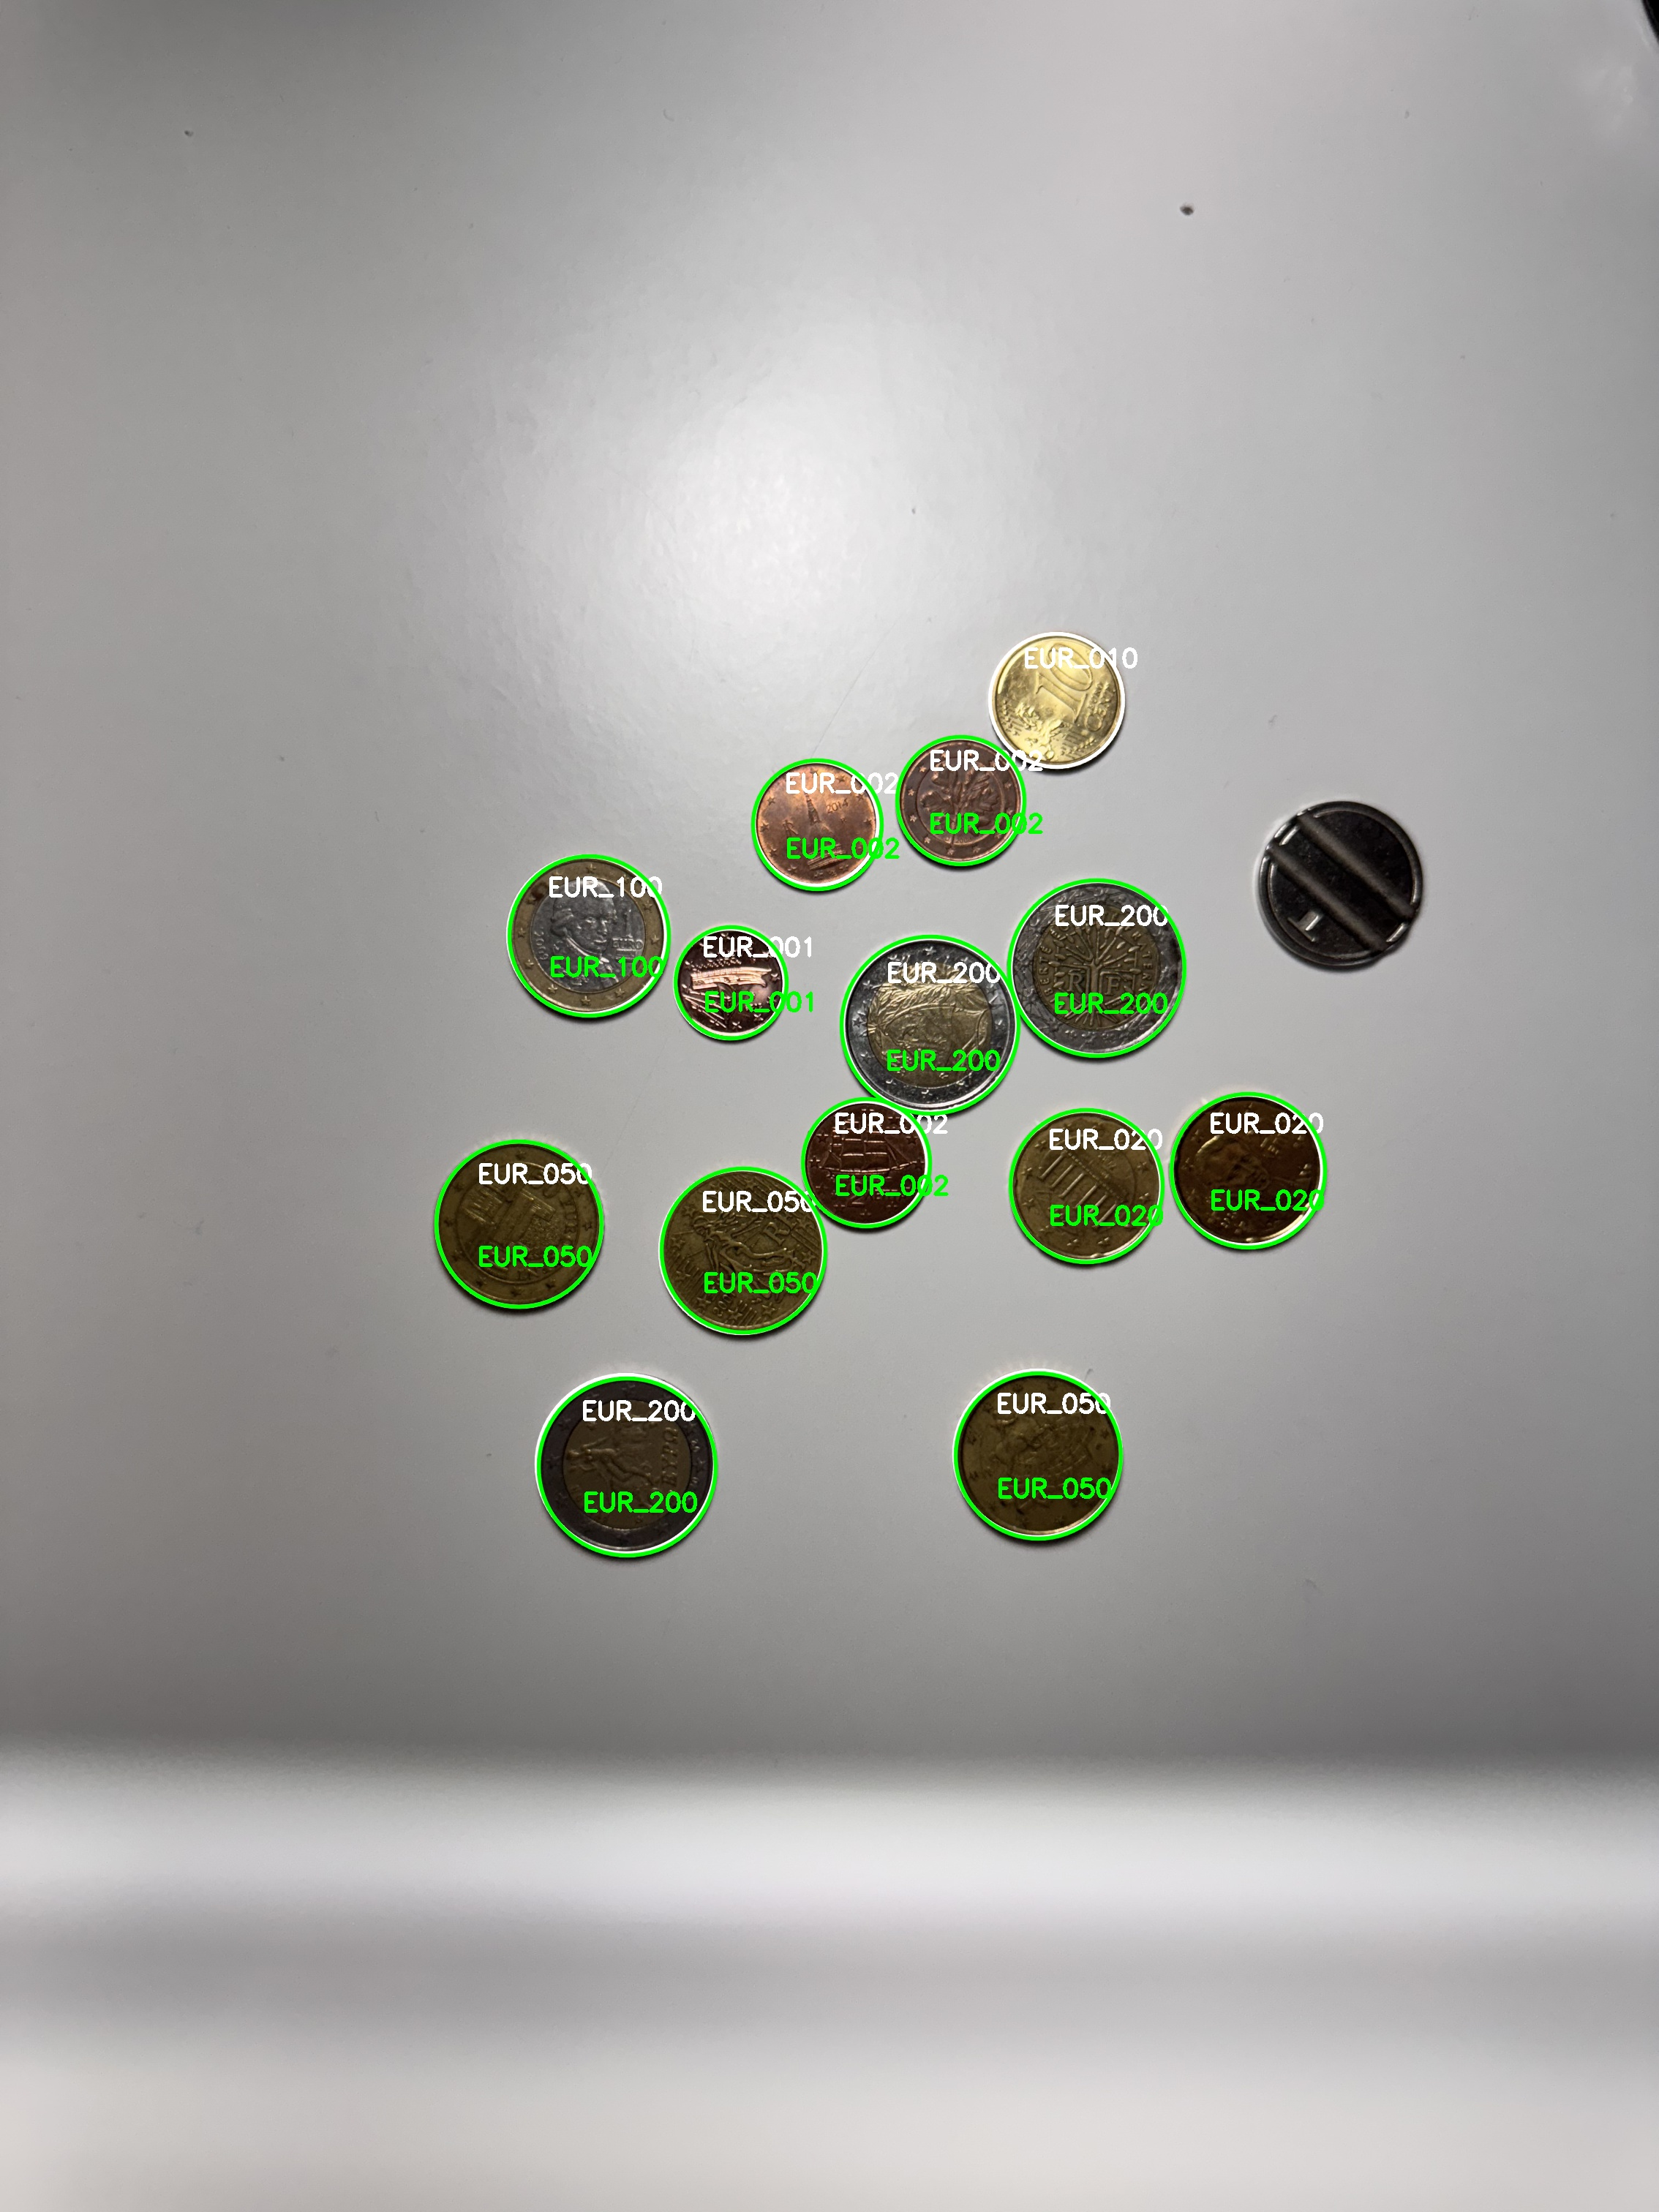
\includegraphics[width=0.45\textwidth]{Immagini/image_0.jpg}
    }\hfill
    \subfloat[\label{Results:fig:image1}]{
        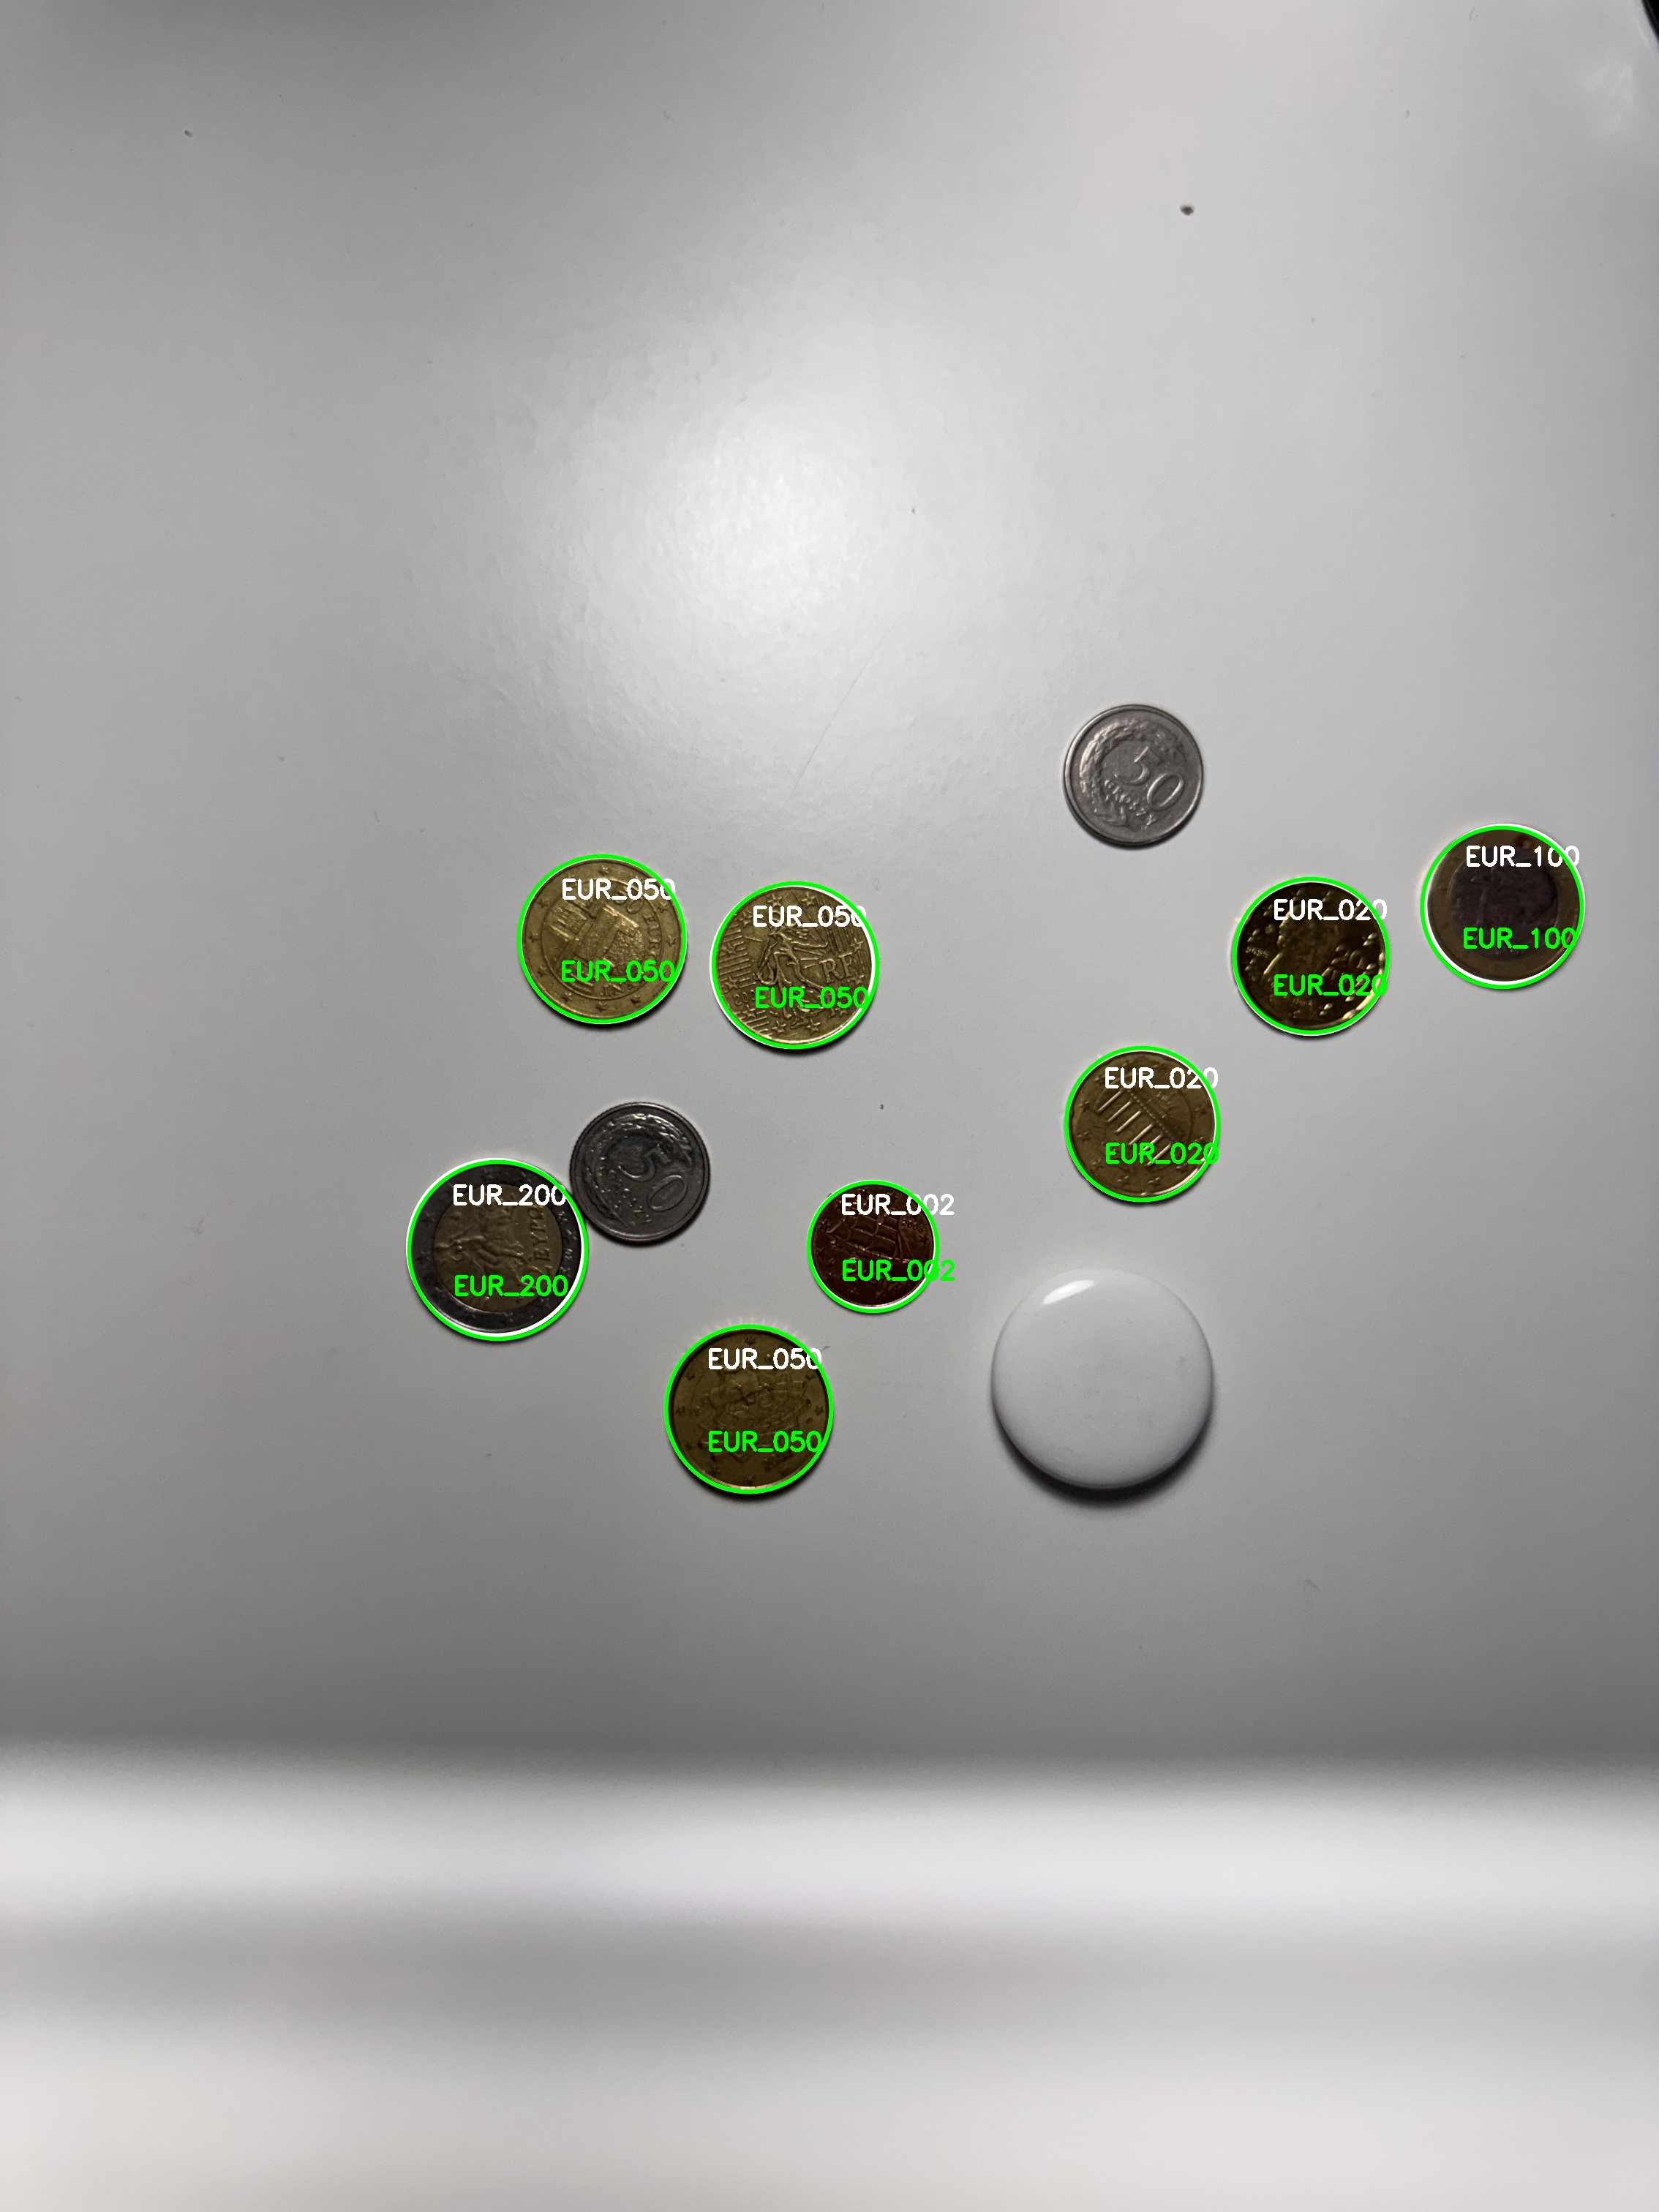
\includegraphics[width=0.45\textwidth]{Immagini/image_1.jpg}
    }
\end{figure}
\begin{figure}[H]
    \ContinuedFloat
    \centering
    \subfloat[\label{Results:fig:image2}]{
        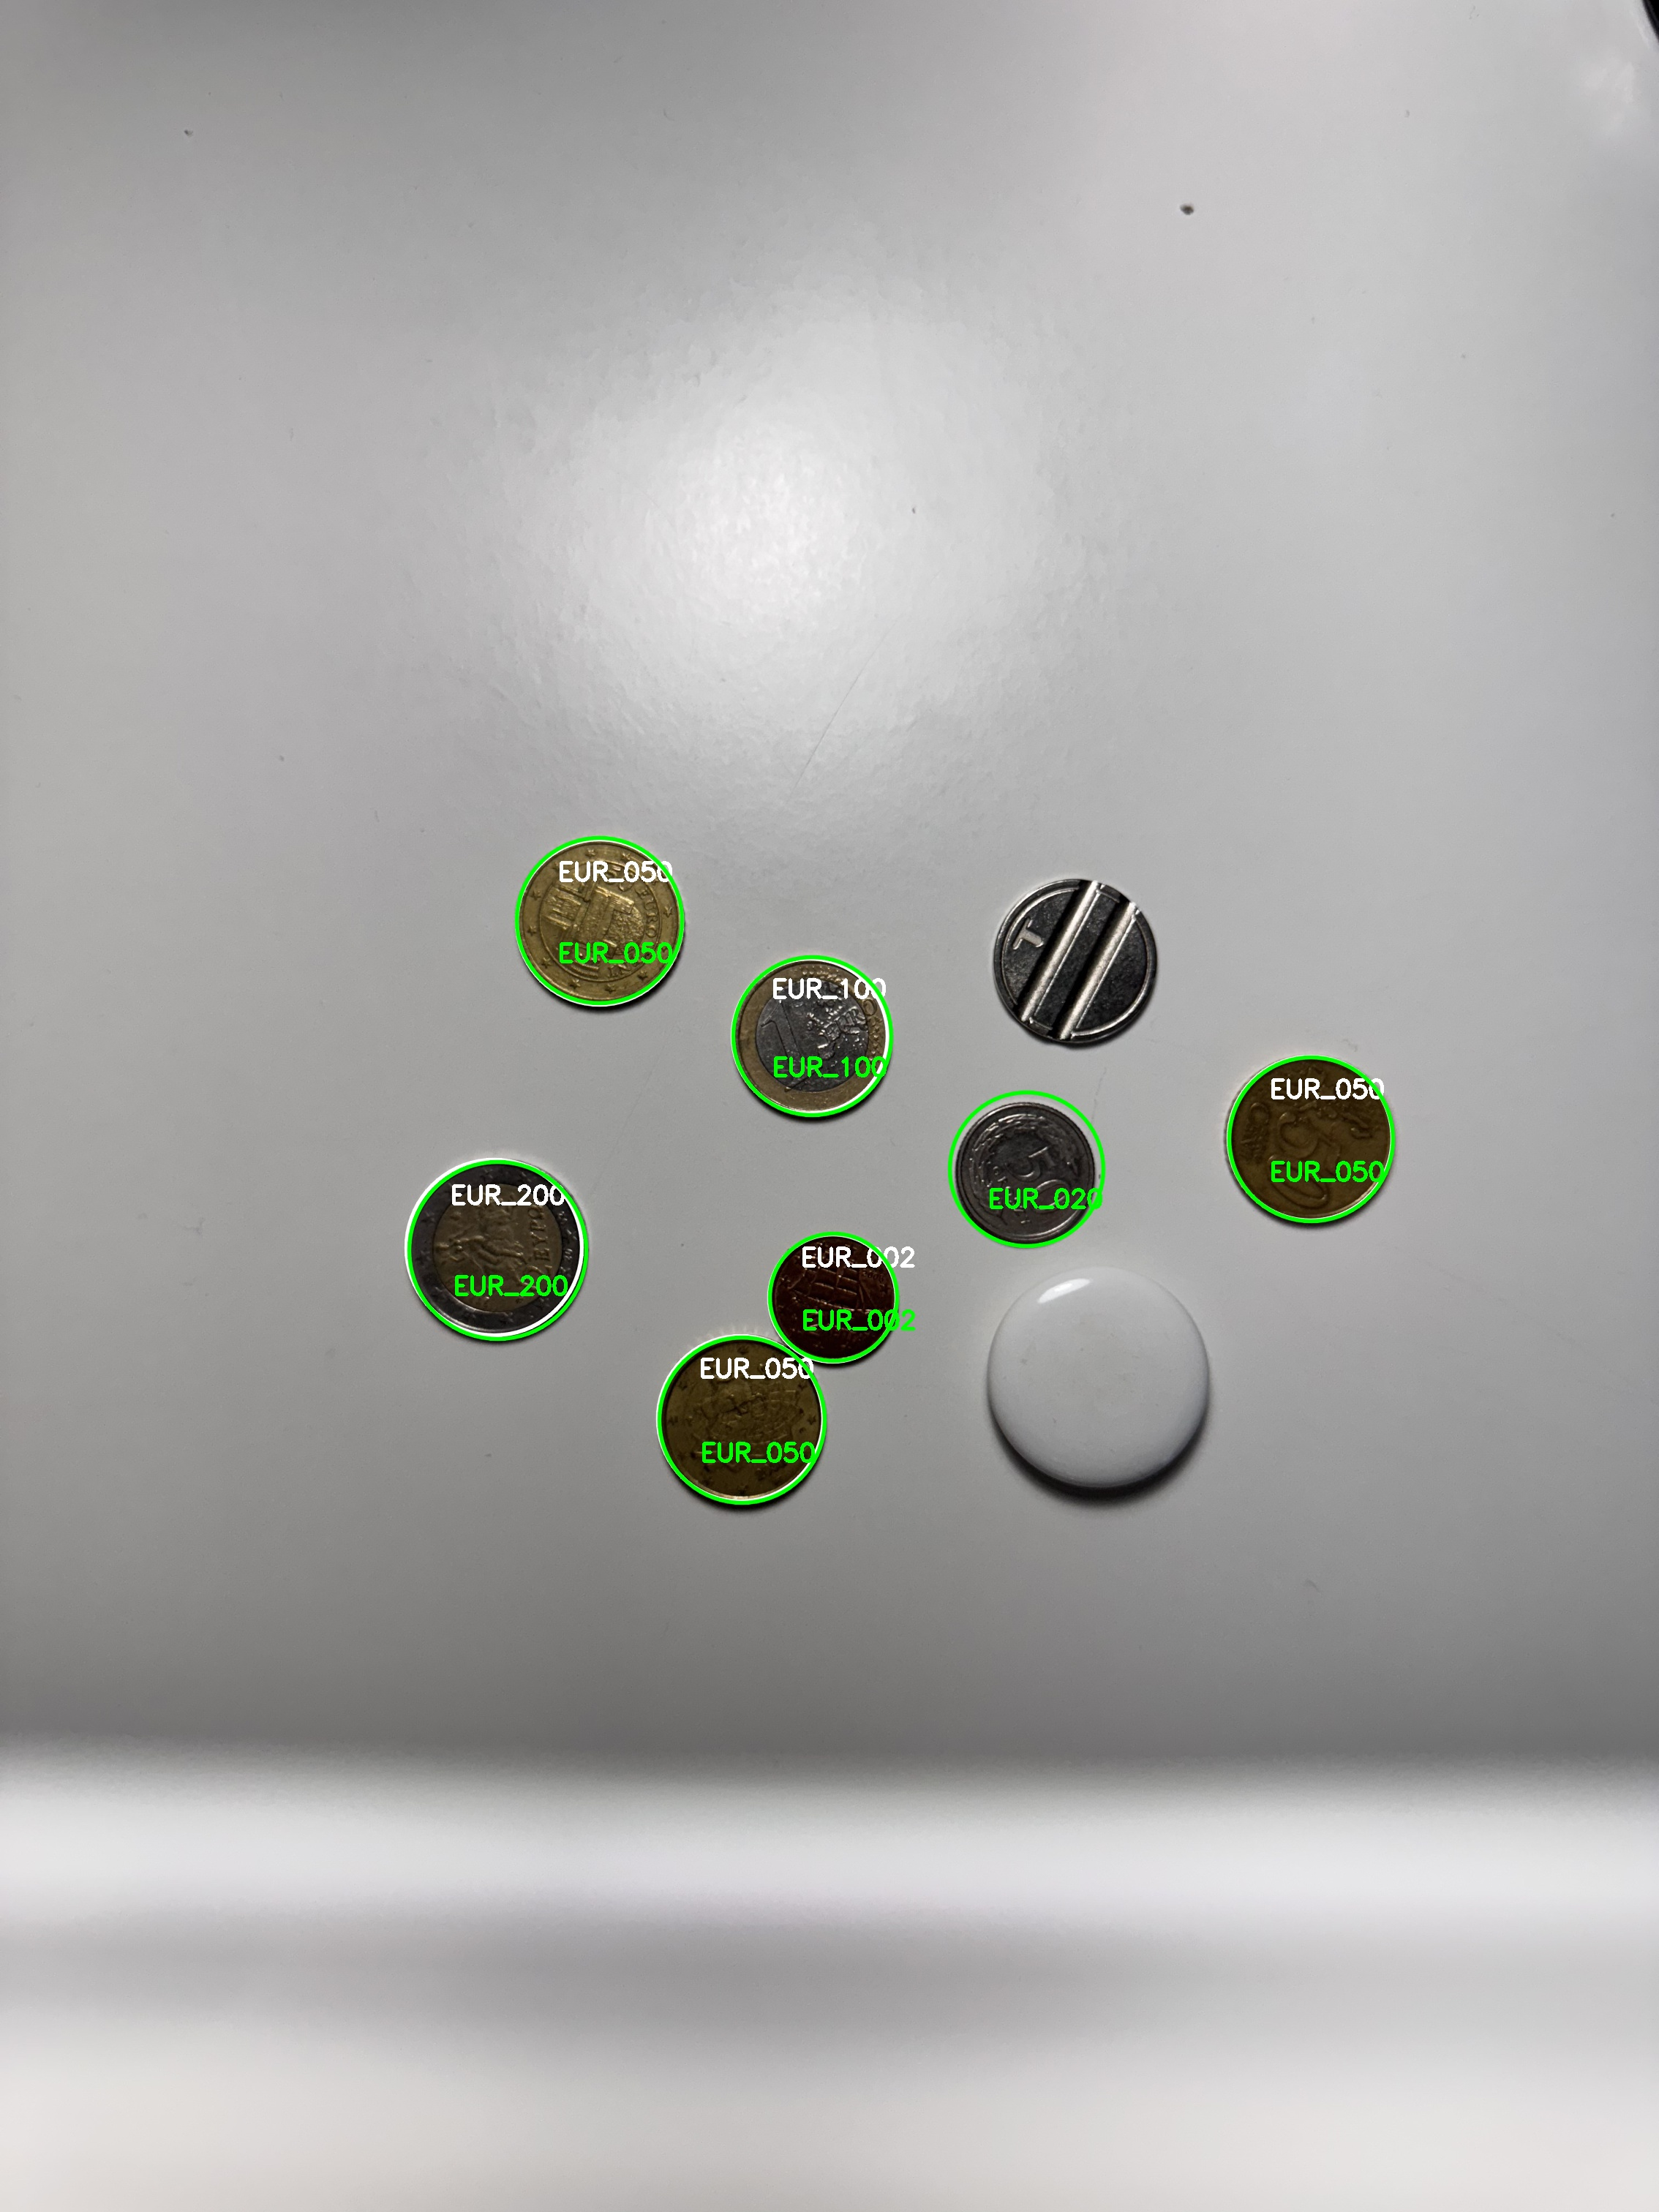
\includegraphics[width=0.45\textwidth]{Immagini/image_2.jpg}
    }\hfill
    \subfloat[\label{Results:fig:image3}]{
        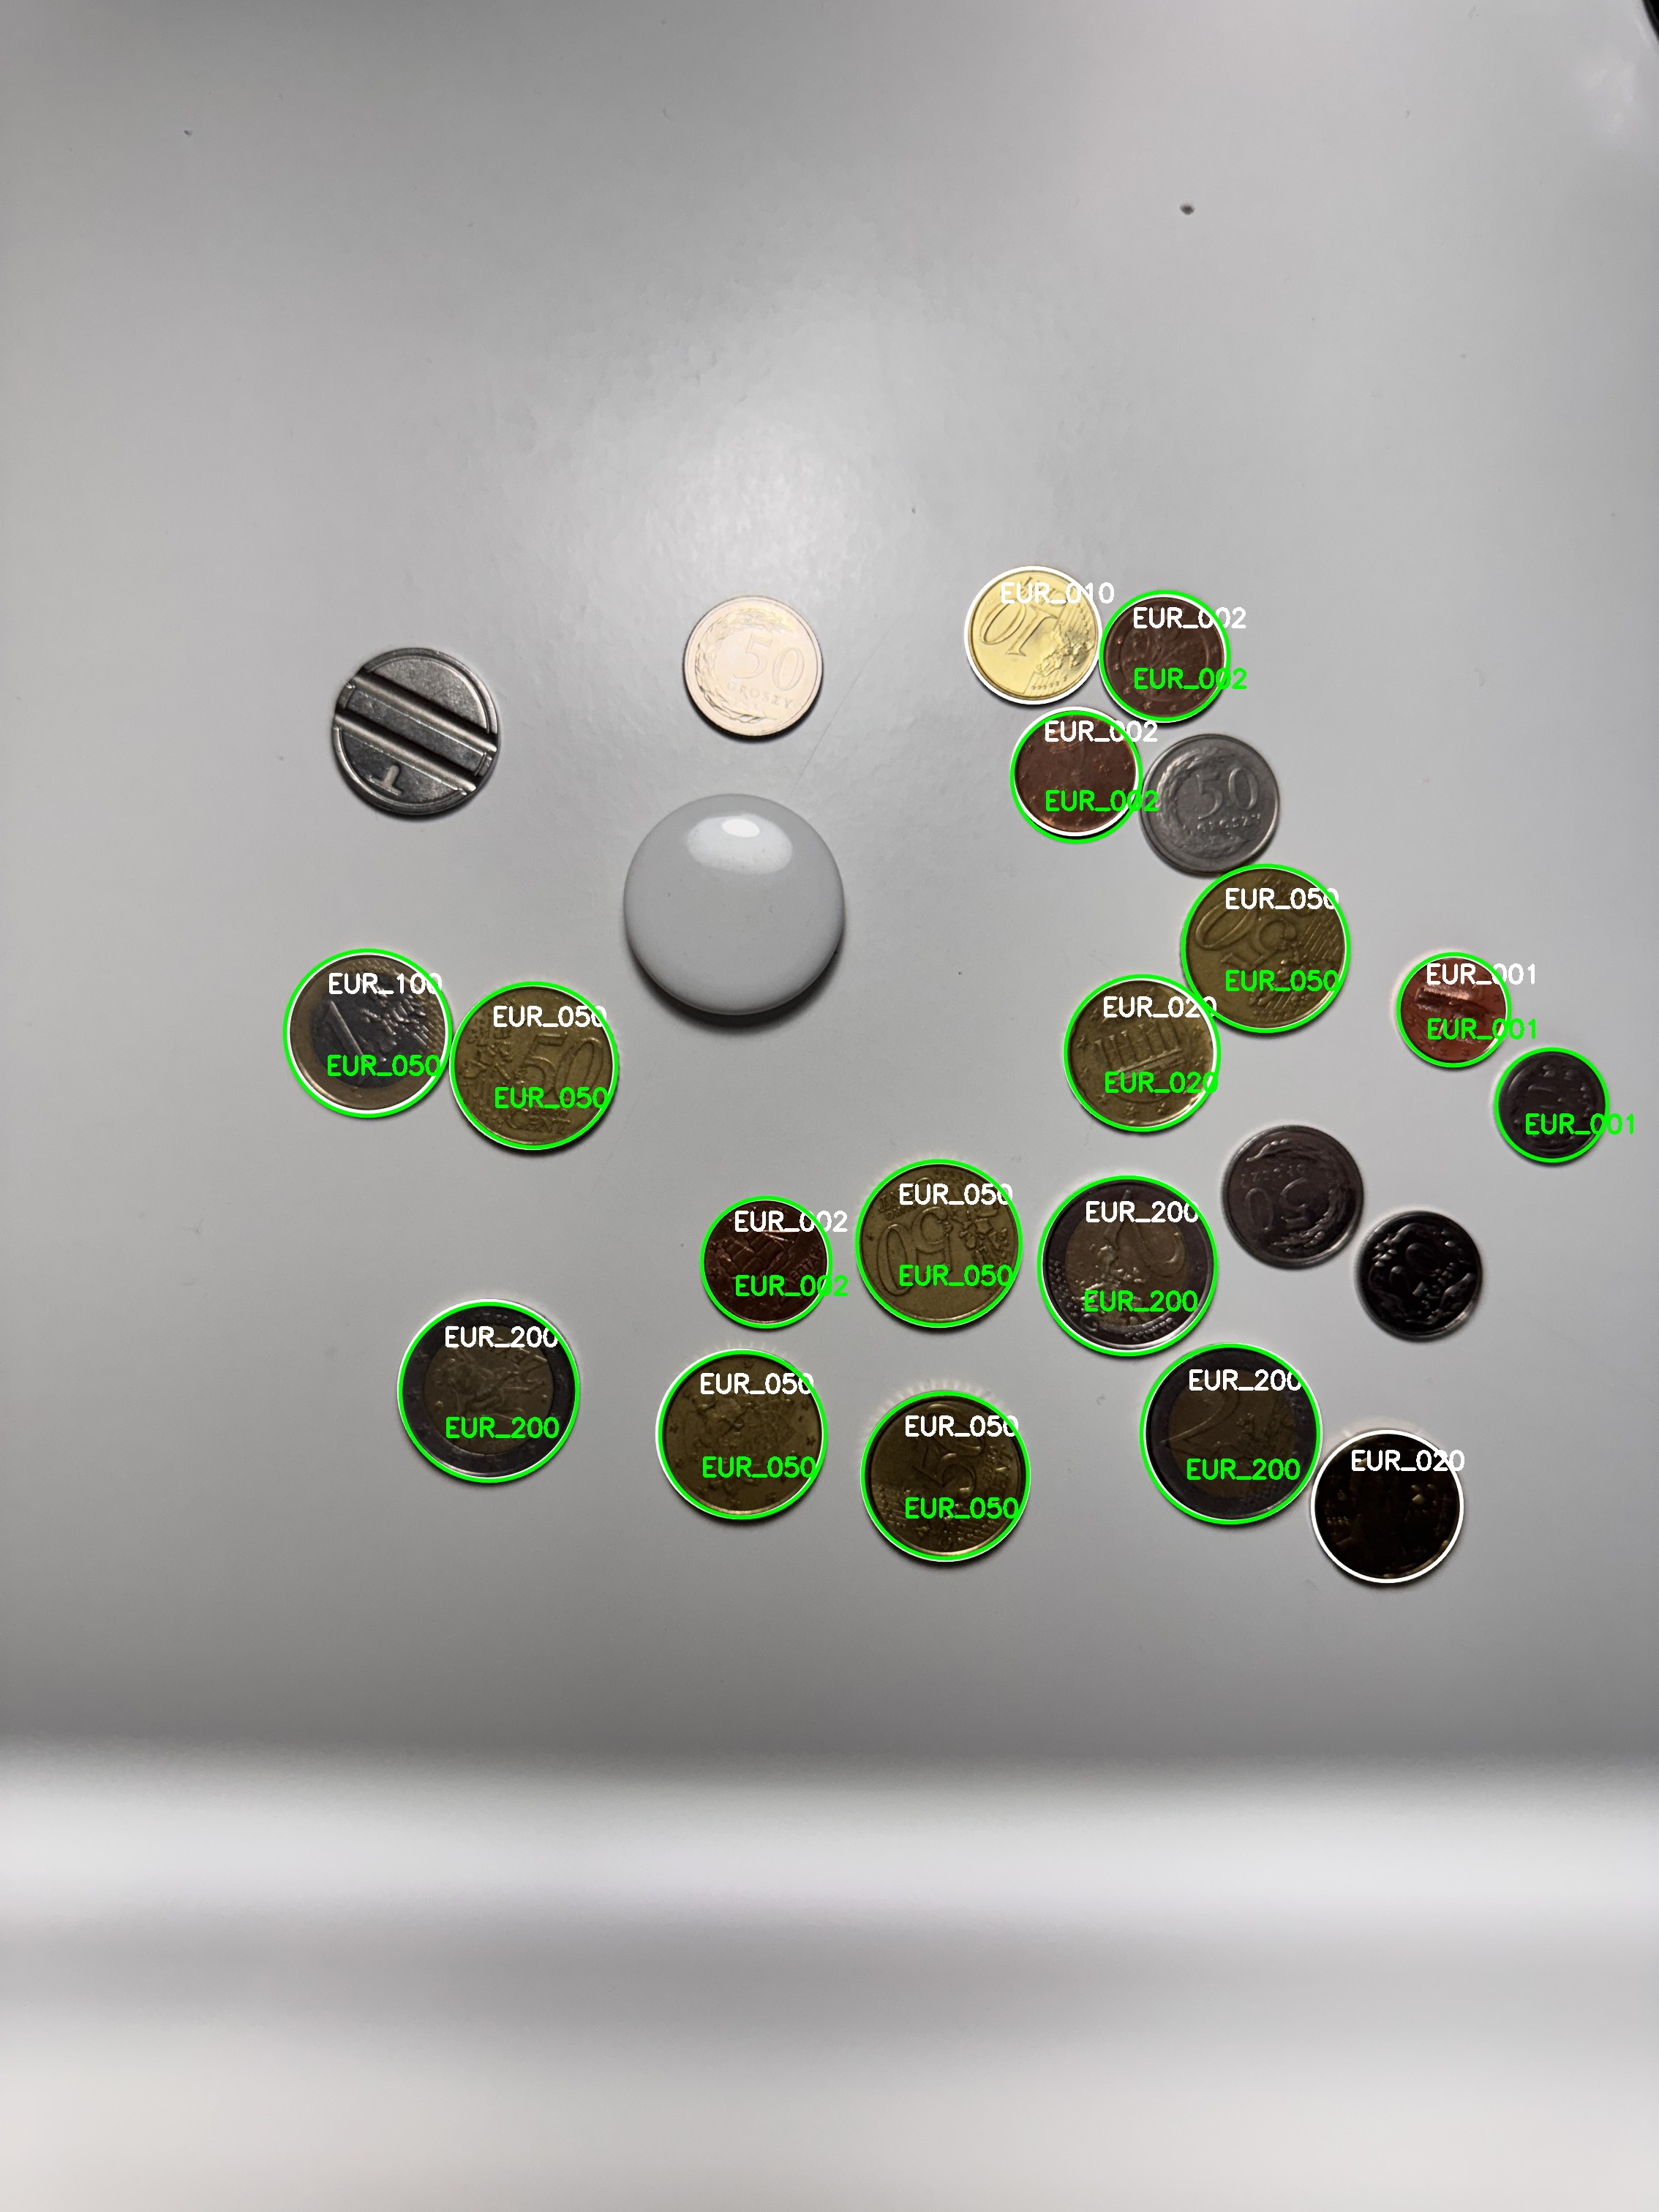
\includegraphics[width=0.45\textwidth]{Immagini/image_3.jpg}
    }
    \addtocounter{figure}{1} % per non saltare il numero
    \caption{Results of the detection algorithm on sample images from the test set.
    The ground truth circles are drawn in white, while the detected ones are drawn in green.}
    \label{Results:fig:images}
\end{figure}
